% Options for packages loaded elsewhere
% Options for packages loaded elsewhere
\PassOptionsToPackage{unicode}{hyperref}
\PassOptionsToPackage{hyphens}{url}
\PassOptionsToPackage{dvipsnames,svgnames,x11names}{xcolor}
%
\documentclass[
  letterpaper,
  DIV=11,
  numbers=noendperiod]{scrartcl}
\usepackage{xcolor}
\usepackage{amsmath,amssymb}
\setcounter{secnumdepth}{-\maxdimen} % remove section numbering
\usepackage{iftex}
\ifPDFTeX
  \usepackage[T1]{fontenc}
  \usepackage[utf8]{inputenc}
  \usepackage{textcomp} % provide euro and other symbols
\else % if luatex or xetex
  \usepackage{unicode-math} % this also loads fontspec
  \defaultfontfeatures{Scale=MatchLowercase}
  \defaultfontfeatures[\rmfamily]{Ligatures=TeX,Scale=1}
\fi
\usepackage{lmodern}
\ifPDFTeX\else
  % xetex/luatex font selection
\fi
% Use upquote if available, for straight quotes in verbatim environments
\IfFileExists{upquote.sty}{\usepackage{upquote}}{}
\IfFileExists{microtype.sty}{% use microtype if available
  \usepackage[]{microtype}
  \UseMicrotypeSet[protrusion]{basicmath} % disable protrusion for tt fonts
}{}
\makeatletter
\@ifundefined{KOMAClassName}{% if non-KOMA class
  \IfFileExists{parskip.sty}{%
    \usepackage{parskip}
  }{% else
    \setlength{\parindent}{0pt}
    \setlength{\parskip}{6pt plus 2pt minus 1pt}}
}{% if KOMA class
  \KOMAoptions{parskip=half}}
\makeatother
% Make \paragraph and \subparagraph free-standing
\makeatletter
\ifx\paragraph\undefined\else
  \let\oldparagraph\paragraph
  \renewcommand{\paragraph}{
    \@ifstar
      \xxxParagraphStar
      \xxxParagraphNoStar
  }
  \newcommand{\xxxParagraphStar}[1]{\oldparagraph*{#1}\mbox{}}
  \newcommand{\xxxParagraphNoStar}[1]{\oldparagraph{#1}\mbox{}}
\fi
\ifx\subparagraph\undefined\else
  \let\oldsubparagraph\subparagraph
  \renewcommand{\subparagraph}{
    \@ifstar
      \xxxSubParagraphStar
      \xxxSubParagraphNoStar
  }
  \newcommand{\xxxSubParagraphStar}[1]{\oldsubparagraph*{#1}\mbox{}}
  \newcommand{\xxxSubParagraphNoStar}[1]{\oldsubparagraph{#1}\mbox{}}
\fi
\makeatother

\usepackage{color}
\usepackage{fancyvrb}
\newcommand{\VerbBar}{|}
\newcommand{\VERB}{\Verb[commandchars=\\\{\}]}
\DefineVerbatimEnvironment{Highlighting}{Verbatim}{commandchars=\\\{\}}
% Add ',fontsize=\small' for more characters per line
\usepackage{framed}
\definecolor{shadecolor}{RGB}{241,243,245}
\newenvironment{Shaded}{\begin{snugshade}}{\end{snugshade}}
\newcommand{\AlertTok}[1]{\textcolor[rgb]{0.68,0.00,0.00}{#1}}
\newcommand{\AnnotationTok}[1]{\textcolor[rgb]{0.37,0.37,0.37}{#1}}
\newcommand{\AttributeTok}[1]{\textcolor[rgb]{0.40,0.45,0.13}{#1}}
\newcommand{\BaseNTok}[1]{\textcolor[rgb]{0.68,0.00,0.00}{#1}}
\newcommand{\BuiltInTok}[1]{\textcolor[rgb]{0.00,0.23,0.31}{#1}}
\newcommand{\CharTok}[1]{\textcolor[rgb]{0.13,0.47,0.30}{#1}}
\newcommand{\CommentTok}[1]{\textcolor[rgb]{0.37,0.37,0.37}{#1}}
\newcommand{\CommentVarTok}[1]{\textcolor[rgb]{0.37,0.37,0.37}{\textit{#1}}}
\newcommand{\ConstantTok}[1]{\textcolor[rgb]{0.56,0.35,0.01}{#1}}
\newcommand{\ControlFlowTok}[1]{\textcolor[rgb]{0.00,0.23,0.31}{\textbf{#1}}}
\newcommand{\DataTypeTok}[1]{\textcolor[rgb]{0.68,0.00,0.00}{#1}}
\newcommand{\DecValTok}[1]{\textcolor[rgb]{0.68,0.00,0.00}{#1}}
\newcommand{\DocumentationTok}[1]{\textcolor[rgb]{0.37,0.37,0.37}{\textit{#1}}}
\newcommand{\ErrorTok}[1]{\textcolor[rgb]{0.68,0.00,0.00}{#1}}
\newcommand{\ExtensionTok}[1]{\textcolor[rgb]{0.00,0.23,0.31}{#1}}
\newcommand{\FloatTok}[1]{\textcolor[rgb]{0.68,0.00,0.00}{#1}}
\newcommand{\FunctionTok}[1]{\textcolor[rgb]{0.28,0.35,0.67}{#1}}
\newcommand{\ImportTok}[1]{\textcolor[rgb]{0.00,0.46,0.62}{#1}}
\newcommand{\InformationTok}[1]{\textcolor[rgb]{0.37,0.37,0.37}{#1}}
\newcommand{\KeywordTok}[1]{\textcolor[rgb]{0.00,0.23,0.31}{\textbf{#1}}}
\newcommand{\NormalTok}[1]{\textcolor[rgb]{0.00,0.23,0.31}{#1}}
\newcommand{\OperatorTok}[1]{\textcolor[rgb]{0.37,0.37,0.37}{#1}}
\newcommand{\OtherTok}[1]{\textcolor[rgb]{0.00,0.23,0.31}{#1}}
\newcommand{\PreprocessorTok}[1]{\textcolor[rgb]{0.68,0.00,0.00}{#1}}
\newcommand{\RegionMarkerTok}[1]{\textcolor[rgb]{0.00,0.23,0.31}{#1}}
\newcommand{\SpecialCharTok}[1]{\textcolor[rgb]{0.37,0.37,0.37}{#1}}
\newcommand{\SpecialStringTok}[1]{\textcolor[rgb]{0.13,0.47,0.30}{#1}}
\newcommand{\StringTok}[1]{\textcolor[rgb]{0.13,0.47,0.30}{#1}}
\newcommand{\VariableTok}[1]{\textcolor[rgb]{0.07,0.07,0.07}{#1}}
\newcommand{\VerbatimStringTok}[1]{\textcolor[rgb]{0.13,0.47,0.30}{#1}}
\newcommand{\WarningTok}[1]{\textcolor[rgb]{0.37,0.37,0.37}{\textit{#1}}}

\usepackage{longtable,booktabs,array}
\usepackage{calc} % for calculating minipage widths
% Correct order of tables after \paragraph or \subparagraph
\usepackage{etoolbox}
\makeatletter
\patchcmd\longtable{\par}{\if@noskipsec\mbox{}\fi\par}{}{}
\makeatother
% Allow footnotes in longtable head/foot
\IfFileExists{footnotehyper.sty}{\usepackage{footnotehyper}}{\usepackage{footnote}}
\makesavenoteenv{longtable}
\usepackage{graphicx}
\makeatletter
\newsavebox\pandoc@box
\newcommand*\pandocbounded[1]{% scales image to fit in text height/width
  \sbox\pandoc@box{#1}%
  \Gscale@div\@tempa{\textheight}{\dimexpr\ht\pandoc@box+\dp\pandoc@box\relax}%
  \Gscale@div\@tempb{\linewidth}{\wd\pandoc@box}%
  \ifdim\@tempb\p@<\@tempa\p@\let\@tempa\@tempb\fi% select the smaller of both
  \ifdim\@tempa\p@<\p@\scalebox{\@tempa}{\usebox\pandoc@box}%
  \else\usebox{\pandoc@box}%
  \fi%
}
% Set default figure placement to htbp
\def\fps@figure{htbp}
\makeatother





\setlength{\emergencystretch}{3em} % prevent overfull lines

\providecommand{\tightlist}{%
  \setlength{\itemsep}{0pt}\setlength{\parskip}{0pt}}



 


\KOMAoption{captions}{tableheading}
\makeatletter
\@ifpackageloaded{tcolorbox}{}{\usepackage[skins,breakable]{tcolorbox}}
\@ifpackageloaded{fontawesome5}{}{\usepackage{fontawesome5}}
\definecolor{quarto-callout-color}{HTML}{909090}
\definecolor{quarto-callout-note-color}{HTML}{0758E5}
\definecolor{quarto-callout-important-color}{HTML}{CC1914}
\definecolor{quarto-callout-warning-color}{HTML}{EB9113}
\definecolor{quarto-callout-tip-color}{HTML}{00A047}
\definecolor{quarto-callout-caution-color}{HTML}{FC5300}
\definecolor{quarto-callout-color-frame}{HTML}{acacac}
\definecolor{quarto-callout-note-color-frame}{HTML}{4582ec}
\definecolor{quarto-callout-important-color-frame}{HTML}{d9534f}
\definecolor{quarto-callout-warning-color-frame}{HTML}{f0ad4e}
\definecolor{quarto-callout-tip-color-frame}{HTML}{02b875}
\definecolor{quarto-callout-caution-color-frame}{HTML}{fd7e14}
\makeatother
\makeatletter
\@ifpackageloaded{caption}{}{\usepackage{caption}}
\AtBeginDocument{%
\ifdefined\contentsname
  \renewcommand*\contentsname{Table of contents}
\else
  \newcommand\contentsname{Table of contents}
\fi
\ifdefined\listfigurename
  \renewcommand*\listfigurename{List of Figures}
\else
  \newcommand\listfigurename{List of Figures}
\fi
\ifdefined\listtablename
  \renewcommand*\listtablename{List of Tables}
\else
  \newcommand\listtablename{List of Tables}
\fi
\ifdefined\figurename
  \renewcommand*\figurename{Figure}
\else
  \newcommand\figurename{Figure}
\fi
\ifdefined\tablename
  \renewcommand*\tablename{Table}
\else
  \newcommand\tablename{Table}
\fi
}
\@ifpackageloaded{float}{}{\usepackage{float}}
\floatstyle{ruled}
\@ifundefined{c@chapter}{\newfloat{codelisting}{h}{lop}}{\newfloat{codelisting}{h}{lop}[chapter]}
\floatname{codelisting}{Listing}
\newcommand*\listoflistings{\listof{codelisting}{List of Listings}}
\makeatother
\makeatletter
\makeatother
\makeatletter
\@ifpackageloaded{caption}{}{\usepackage{caption}}
\@ifpackageloaded{subcaption}{}{\usepackage{subcaption}}
\makeatother
\usepackage{bookmark}
\IfFileExists{xurl.sty}{\usepackage{xurl}}{} % add URL line breaks if available
\urlstyle{same}
\hypersetup{
  pdftitle={Chapter 7 - Normal approximation: Exercise solutions},
  pdfauthor={Mattias Villani},
  colorlinks=true,
  linkcolor={blue},
  filecolor={Maroon},
  citecolor={Blue},
  urlcolor={Blue},
  pdfcreator={LaTeX via pandoc}}


\title{Chapter 7 - Normal approximation: Exercise solutions}
\author{Mattias Villani}
\date{}
\begin{document}
\maketitle


Click on the arrow to see a solution.

\subsubsection{Exercise 7.1}\label{exercise-7.1}

The dataset \texttt{ebay.csv} available at
\url{https://github.com/mattiasvillani/BayesianLearningBook/raw/main/data/ebaybids.csv}
contains the final selling price (\texttt{FinalPrice}) in \(1000\) eBay
auctions for collectors coins. We will here only consider the final
price of the sold coins, and we discard the auctions with unsold coins
(\texttt{FinalPrice}=NA) and the single auction with
\texttt{FinalPrice}\(=0\). We model the final price \(Y_i\) in auction
\(i\) using a Gamma distribution \begin{equation*}
   Y_i \vert \alpha,\beta \sim \mathrm{Gamma}(\alpha,\beta),
  \end{equation*} where \(\alpha>0\) is the shape parameter and
\(\beta>0\) is the rate parameter. Our aim is the posterior distribution
\(p(\alpha, \beta \vert \mathbf{y})\) conditional on the data
\(\mathbf{y}\), the selling prices in the auctions with at least one
bidder. Since both parameters are strictly positive we re-parameterize
the model using the exponential function \begin{align*}
    \alpha &= \exp(\theta_1)\\
    \beta &= \exp(\theta_2).
  \end{align*} where both \(\theta_1\) and \(\theta_2\) are free to take
on any value in \((-\infty,\infty)\). Use the prior \begin{align*}
    \theta_1 &\sim N(0, \tau^2)\\
    \theta_2 &\sim N(0, \tau^2)
  \end{align*} and we set \(\tau=10\) to get a weakly informative prior.

\begin{enumerate}[(a)]
    \item   \input{exercises/normalapprox/gamma_approx_a.tex}
    \item   \input{exercises/normalapprox/gamma_approx_b.tex}
\end{enumerate}

We start off by loading the data:

\begin{Shaded}
\begin{Highlighting}[]
\NormalTok{data }\OtherTok{=} \FunctionTok{read.csv}\NormalTok{(}\StringTok{"https://raw.githubusercontent.com/mattiasvillani/BayesianLearningBook/main/data/ebaybids.csv"}\NormalTok{)}
\NormalTok{y }\OtherTok{=}\NormalTok{ data}\SpecialCharTok{$}\NormalTok{FinalPrice[}\SpecialCharTok{!}\FunctionTok{is.na}\NormalTok{(data}\SpecialCharTok{$}\NormalTok{FinalPrice) }\SpecialCharTok{\&}\NormalTok{ (data}\SpecialCharTok{$}\NormalTok{FinalPrice}\SpecialCharTok{\textgreater{}}\DecValTok{0}\NormalTok{)]}
\FunctionTok{hist}\NormalTok{(y, }\DecValTok{30}\NormalTok{, }\AttributeTok{freq =} \ConstantTok{FALSE}\NormalTok{, }\AttributeTok{col =}\StringTok{"cornsilk"}\NormalTok{, }
     \AttributeTok{xlab =} \StringTok{"Final price"}\NormalTok{, }\AttributeTok{ylab =} \StringTok{"density"}\NormalTok{, }\AttributeTok{main =} \StringTok{""}\NormalTok{)}
\end{Highlighting}
\end{Shaded}

\pandocbounded{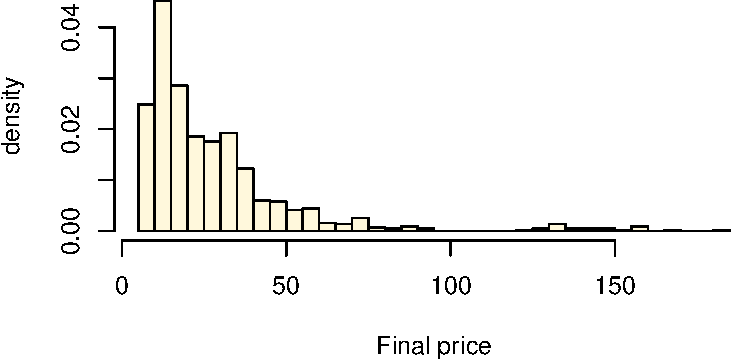
\includegraphics[keepaspectratio]{ch7solutions_files/figure-pdf/unnamed-chunk-2-1.pdf}}

\textbf{a)} Determine a normal approximation of the posterior
distribution \(p(\boldsymbol{\theta} | \mathbf{y})\) based on numerical
optimization, where \(\boldsymbol{\theta} = (\theta_1,\theta_2)^\top\).

\begin{tcolorbox}[enhanced jigsaw, opacityback=0, bottomrule=.15mm, title={Solution}, colback=white, colframe=quarto-callout-note-color-frame, breakable, toprule=.15mm, arc=.35mm, bottomtitle=1mm, left=2mm, coltitle=black, colbacktitle=quarto-callout-note-color!10!white, titlerule=0mm, rightrule=.15mm, toptitle=1mm, leftrule=.75mm, opacitybacktitle=0.6]

We use the normal approximation suggested by the Bernstein-von Mises
theorem: \[
\boldsymbol{\theta} \overset{\mathrm{approx}}{\sim} N(\tilde{\boldsymbol{\theta}}, \boldsymbol{J}^{-1}_{\mathbf{y}})
\] where the posterior mode \(\tilde{\boldsymbol{\theta}}\) and
posterior information matrix \(\boldsymbol{J}^{-1}_{\mathbf{y}}\) are
obtained by numerical optimization. To use optim in R we need to code up
the log posterior function

\begin{Shaded}
\begin{Highlighting}[]
\NormalTok{logPostGamma }\OtherTok{\textless{}{-}} \ControlFlowTok{function}\NormalTok{(theta, y, tau)\{}
\NormalTok{  alpha }\OtherTok{=} \FunctionTok{exp}\NormalTok{(theta[}\DecValTok{1}\NormalTok{])}
\NormalTok{  beta\_ }\OtherTok{=} \FunctionTok{exp}\NormalTok{(theta[}\DecValTok{2}\NormalTok{])}
\NormalTok{  logLik }\OtherTok{=} \FunctionTok{sum}\NormalTok{(}\FunctionTok{dgamma}\NormalTok{(y, alpha, beta\_, }\AttributeTok{log =} \ConstantTok{TRUE}\NormalTok{))}
\NormalTok{  logPrior }\OtherTok{=} \FunctionTok{dnorm}\NormalTok{(}\DecValTok{0}\NormalTok{, tau, }\AttributeTok{log =} \ConstantTok{TRUE}\NormalTok{) }\SpecialCharTok{+} \FunctionTok{dnorm}\NormalTok{(}\DecValTok{0}\NormalTok{, tau, }\AttributeTok{log =} \ConstantTok{TRUE}\NormalTok{)}
  \FunctionTok{return}\NormalTok{(logLik }\SpecialCharTok{+}\NormalTok{ logPrior)}
\NormalTok{\}}
\end{Highlighting}
\end{Shaded}

We can then find all the quantities needed for the normal approximation
by running optim.

\begin{Shaded}
\begin{Highlighting}[]
\NormalTok{tau }\OtherTok{=} \DecValTok{10}
\NormalTok{initVal }\OtherTok{\textless{}{-}} \FunctionTok{c}\NormalTok{(}\DecValTok{0}\NormalTok{,}\DecValTok{0}\NormalTok{) }\CommentTok{\# these initial values imply a Gamma(1,1) distribution.}
\NormalTok{OptimResults}\OtherTok{\textless{}{-}}\FunctionTok{optim}\NormalTok{(initVal, logPostGamma, }\AttributeTok{gr=}\ConstantTok{NULL}\NormalTok{, y[}\DecValTok{1}\SpecialCharTok{:}\DecValTok{260}\NormalTok{], tau,}
  \AttributeTok{method =} \FunctionTok{c}\NormalTok{(}\StringTok{"BFGS"}\NormalTok{), }\AttributeTok{control =} \FunctionTok{list}\NormalTok{(}\AttributeTok{fnscale=}\SpecialCharTok{{-}}\DecValTok{1}\NormalTok{), }\AttributeTok{hessian=}\ConstantTok{TRUE}\NormalTok{)}
\NormalTok{postMode }\OtherTok{=}\NormalTok{ OptimResults}\SpecialCharTok{$}\NormalTok{par}
\NormalTok{postCov }\OtherTok{=} \SpecialCharTok{{-}}\FunctionTok{solve}\NormalTok{(OptimResults}\SpecialCharTok{$}\NormalTok{hessian)}
\end{Highlighting}
\end{Shaded}

The normal posterior approximation thus has mean vector

\begin{Shaded}
\begin{Highlighting}[]
\NormalTok{postMode}
\end{Highlighting}
\end{Shaded}

\begin{verbatim}
[1]  0.695345 -2.577673
\end{verbatim}

and covariance matrix

\begin{Shaded}
\begin{Highlighting}[]
\NormalTok{postCov}
\end{Highlighting}
\end{Shaded}

\begin{verbatim}
           [,1]        [,2]
[1,] 0.00663615 0.006636150
[2,] 0.00663615 0.008555005
\end{verbatim}

from which we can compute the approximate posterior standard deviations:

\begin{Shaded}
\begin{Highlighting}[]
\NormalTok{postStd }\OtherTok{=} \FunctionTok{sqrt}\NormalTok{(}\FunctionTok{diag}\NormalTok{(postCov))}
\end{Highlighting}
\end{Shaded}

\end{tcolorbox}

\textbf{b)} Combine the approximation from a) and simulation to
approximate the marginal posterior for the original parameters
\(\alpha\) and \(\beta\), as well as the marginal posterior of the mean
\(\alpha/\beta\) and standard deviation \(\sqrt{\alpha}/\beta\) of the
fitted Gamma distribution.

\begin{tcolorbox}[enhanced jigsaw, opacityback=0, bottomrule=.15mm, title={Solution}, colback=white, colframe=quarto-callout-note-color-frame, breakable, toprule=.15mm, arc=.35mm, bottomtitle=1mm, left=2mm, coltitle=black, colbacktitle=quarto-callout-note-color!10!white, titlerule=0mm, rightrule=.15mm, toptitle=1mm, leftrule=.75mm, opacitybacktitle=0.6]

We use the \texttt{mvtnorm} package to simulate from the normal
approximation and then compute the transformation for each draw for
\(j=1,\ldots,m\): \[
\begin{aligned}
\alpha^{(i)} &= \exp\big(\theta_1^{(i)} \big) \\
\beta^{(i)} &= \exp\big(\theta_2^{(i)} \big)
\end{aligned}
\] We can then further compute the mean \(\alpha/\beta\) and standard
deviation \(\sqrt{\alpha}/\beta\) for each draw. Here is the code:

\begin{Shaded}
\begin{Highlighting}[]
\FunctionTok{library}\NormalTok{(mvtnorm)}
\NormalTok{nSim }\OtherTok{=} \DecValTok{10000}
\NormalTok{thetaDraws }\OtherTok{=} \FunctionTok{rmvnorm}\NormalTok{(nSim, postMode, postCov)}
\NormalTok{alphaDraws }\OtherTok{=} \FunctionTok{exp}\NormalTok{(thetaDraws[,}\DecValTok{1}\NormalTok{])}
\NormalTok{betaDraws }\OtherTok{=} \FunctionTok{exp}\NormalTok{(thetaDraws[,}\DecValTok{2}\NormalTok{])}
\NormalTok{meanDraws }\OtherTok{=}\NormalTok{ alphaDraws}\SpecialCharTok{/}\NormalTok{betaDraws}
\NormalTok{stdDraws }\OtherTok{=} \FunctionTok{sqrt}\NormalTok{(alphaDraws) }\SpecialCharTok{/}\NormalTok{ betaDraws}
\FunctionTok{par}\NormalTok{(}\AttributeTok{mfrow =} \FunctionTok{c}\NormalTok{(}\DecValTok{2}\NormalTok{,}\DecValTok{2}\NormalTok{))}
\FunctionTok{hist}\NormalTok{(alphaDraws, }\DecValTok{30}\NormalTok{, }\AttributeTok{freq =} \ConstantTok{FALSE}\NormalTok{, }\AttributeTok{main =} \FunctionTok{expression}\NormalTok{(alpha), }
     \AttributeTok{xlab =} \FunctionTok{expression}\NormalTok{(alpha), }\AttributeTok{col =} \StringTok{"cornflowerblue"}\NormalTok{)}
\FunctionTok{hist}\NormalTok{(betaDraws, }\DecValTok{30}\NormalTok{, }\AttributeTok{freq =} \ConstantTok{FALSE}\NormalTok{, }\AttributeTok{main =} \FunctionTok{expression}\NormalTok{(beta), }
     \AttributeTok{xlab =} \FunctionTok{expression}\NormalTok{(beta), }\AttributeTok{col =} \StringTok{"cornflowerblue"}\NormalTok{)}
\FunctionTok{hist}\NormalTok{(meanDraws, }\DecValTok{30}\NormalTok{, }\AttributeTok{freq =} \ConstantTok{FALSE}\NormalTok{, }\AttributeTok{main =} \StringTok{"Expected value"}\NormalTok{, }\AttributeTok{xlab =} \StringTok{"mean"}\NormalTok{, }
     \AttributeTok{col =} \StringTok{"cornsilk"}\NormalTok{)}
\FunctionTok{hist}\NormalTok{(stdDraws, }\DecValTok{30}\NormalTok{, }\AttributeTok{freq =} \ConstantTok{FALSE}\NormalTok{, }\AttributeTok{main =} \StringTok{"Standard deviation"}\NormalTok{, }
     \AttributeTok{xlab =} \StringTok{"st dev"}\NormalTok{, }\AttributeTok{col =} \StringTok{"cornsilk"}\NormalTok{)}
\end{Highlighting}
\end{Shaded}

\pandocbounded{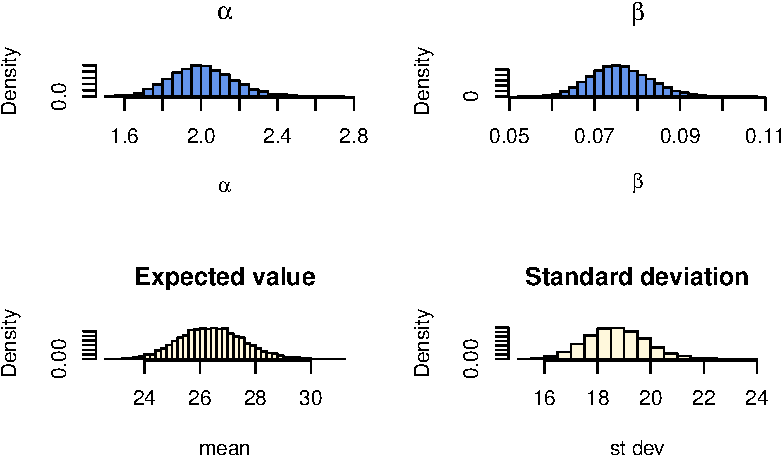
\includegraphics[keepaspectratio]{ch7solutions_files/figure-pdf/unnamed-chunk-8-1.pdf}}

\end{tcolorbox}




\end{document}
